\documentclass{article}

\usepackage{xeCJK}
\usepackage{graphicx}
\usepackage{caption}
\usepackage{subfigure}
\usepackage[colorlinks=true,
linkcolor=blue
]{hyperref}
\usepackage{listings}
\usepackage[outputdir=build]{minted}
\usepackage{amsmath}
\usepackage{lastpage}   %获得总页数
\usepackage{fancyhdr}
\usepackage{bookmark}
\graphicspath{{../img/}}
\pagestyle{fancy}
\setlength{\headheight}{64pt}
\lhead{}
\chead{}
\rhead{}
\lfoot{}
\cfoot{}
\rfoot{\thepage\ of \pageref{LastPage}} % 当前页 of 总页数
\renewcommand{\headrulewidth}{0.4pt}    % 改为0pt即可去掉页眉下面的横线
\renewcommand{\footrulewidth}{0.4pt}    % 改为0pt即可去掉页脚上面的横线
\lhead{
\includegraphics[height=0.8in]{depsast.jpg}}  % 插入科协LOGO
\setCJKfamilyfont{yy}{YouYuan}                       % 幼圆  yy

\newcommand{\yy}{\CJKfamily{yy}}
\renewcommand{\baselinestretch}{1.6}

\makeatletter
\renewcommand\paragraph{\@startsection{paragraph}{4}{\z@}%
            {-2.5ex\@plus -1ex \@minus -.25ex}%
            {1.25ex \@plus .25ex}%
            {\normalfont\normalsize\bfseries}}  % make paragraph act like 'subsubsubsection'
\makeatother
\setcounter{secnumdepth}{4} % how many sectioning levels to assign numbers to
\setcounter{tocdepth}{4}    % how many sectioning levels to show in ToC

\graphicspath{{./img/ccd/}{./img/}}

\begin{document}


\title{6-6 线性CCD模块介绍}
\author{工程物理系学生科协技术部\quad 高一川}
\date{\today}
\maketitle
\tableofcontents
\newpage


\section{前言}
线性 CCD 模块是智能车的“眼睛”,本文档旨在向大家阐述线性 CCD 的基本原理及其软硬件使用说明。

\section{线性 CCD 简介}

\subsection{与面阵 CCD 的区别}

说到 CCD,想必大家都不陌生。在我们常用的手机、数码相机等电子设备的摄像头中,CCD 得到了广泛的应用。但是细心的各位可能发现了,我们这篇文档从始至终都在强调“线性” CCD,那么什么是线性 CCD,它又与我们常说的 CCD 有什么区别呢?

我们常说的 CCD 指的是面阵 CCD,在你使用手机拍照后,会得到一幅图像,如果你感兴趣的话,打开图像的属性可以看到它的尺寸,例如 1920x1080。从此可以发现,手机里面的 CCD 拍下的图像可以被认为是一个 1920x1080 的矩阵(这里只考虑灰度图像)。但是如果你使用线性 CCD 拍摄下同样一幅图像,你会发现它的尺寸是 1x128,也就是说线性 CCD 拍下的图像是一个仅有一个像素宽的长条,我们可以将其作为一个由 128 个灰度值组成的向量(数组),这也就是两种 CCD 最大的不同之处。两种 CCD 拍到的图片如下图所示。

\begin{figure}[h]
 \centering
 \captionsetup{labelformat=empty}
 \begin{minipage}[t]{0.35\textwidth}
  \centering
  
\includegraphics[width=\linewidth]{common_ccd.jpg}
  \caption{\scriptsize{面阵 CCD 拍到的赛道图像}}
 \end{minipage}
 \begin{minipage}[t]{0.35\textwidth}
  \centering
  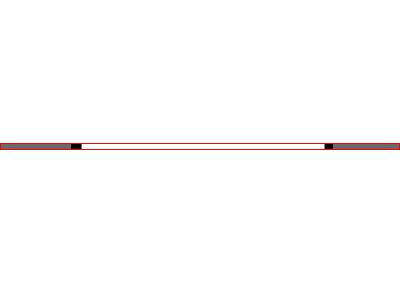
\includegraphics[width=\linewidth]{linear_ccd.jpg}
  \caption{\scriptsize{线性 CCD 拍到的赛道图像}}
 \end{minipage}
\end{figure}

\subsection{模块引脚介绍}

本届智能车大赛提供的线性 CCD 模块的主芯片为 TSL1401CL 芯片,模块共引出了六个引脚,各引脚的功能及其与单片机 IO 口的连接如下表:

\begin{table}[]
 \centering
 \captionsetup{labelformat=empty}
 \caption{线性 CCD 模块引脚功能}
 \label{ccd_pinouts}
 \begin{tabular}{|l|l|l|l|}
  \hline
  引脚序号 & 名称 & 连接的 IO 口 & 功能描述    \\ \hline
  1            & GND    & GND              & 地线          \\
  2            & VDD    & 3V3              & 3.3V 电源     \\
  3            & AO     &                  & 模拟量输出 \\
  4            & CLK    &                  & 时钟输入    \\
  5            & SI     &                  & 串行输入    \\
  6            & AM     & NC               & 无连接       \\ \hline
 \end{tabular}
\end{table}

\subsection{功能及时序描述}

TSL1401 芯片包含 128 个线性排列的光电二极管,同时片内为每个光电二极管集成了独自的积分电路,下面为了便于理解,我们将这些光电二极管及其积分电路统称为像素。对于每个像素来说,其采集到的灰度值均与其感知的光强与积分(曝光)时间成正比,而采集到的灰度值将在 AO 线上以模拟信号(电压)的形式输出,下面将每个像素采集到的灰度值称为其像素值。那么问题来了,我们共有 128 个像素值要传输给单片机,但是 AO 线只有一根,怎么办呢?这时候就轮到 CLK 和 SI 这两个信号上场了。

\begin{figure}[h]
\centering % 使后面的内容居中
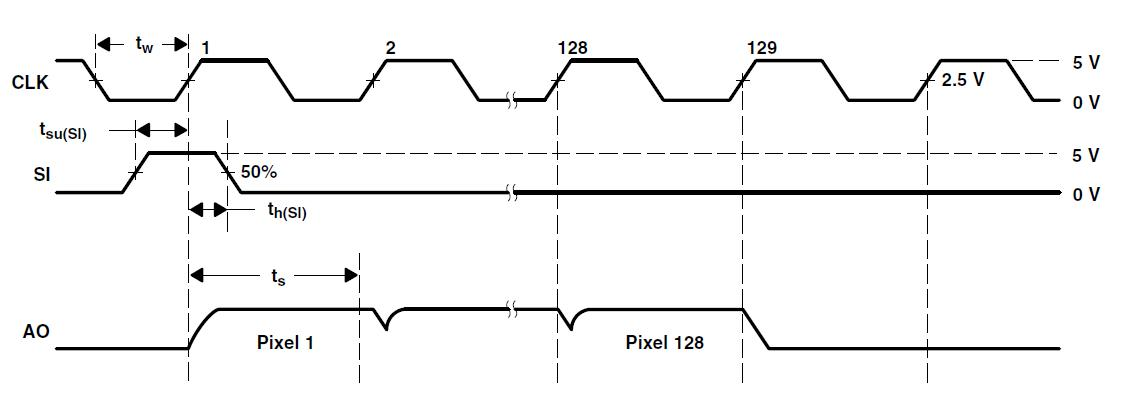
\includegraphics[width=.8\textwidth]{tsl1401_timing.jpg}
\caption{TSL1401 时序图}
\label{tsl1401_timing}
\end{figure}

如果你去查阅 TSL1401 芯片的数据手册,你会看到如图\ref{tsl1401_timing}的时序图。如果这是你第一次查看一款芯片的时序图,你可能已经被这些复杂的波形所迷惑,那么不妨让我们结合单次采集的代码来理解一下这个时序,相信会更加清楚明了。

\begin{minted}[showspaces=false,breaklines=true]{c}
void CCD_getline(uint8 *pixel)
{
  uint8 i;

  /* 以下代码为采集前的曝光处理 */
  TSL1401_SI(1);    // SI 线发送高电平
  CCD_delay();      // 极短的延时(几个时钟周期)
  TSL1401_CLK(1);   // 时钟线发送高电平
  TSL1401_SI(0);    // SI 线发送低电平,此处 CCD 开始曝光
  CCD_delay();      // 第一个时钟信号
  TSL1401_CLK(0);   // 时钟线发送低电平,此时第一个时钟周期结束

  // 发送第 2~129 个时钟信号,此处所需总时间很短,可以忽略不计
  for(i=1; i<129; i++)
  {
    CCD_delay();
    TSL1401_CLK(1);
    CCD_delay();
    TSL1401_CLK(0);
  }

  // CCD 曝光时间的延时,单位为 ms,此处决定了 CCD 在本次采集中实际的曝光时间
  CCD_integration_delay(INT_TIME);

  /* 以下代码为采集上次曝光得到的图像 */
  TSL1401_SI(1);    // 提供初始的 SI 信号
  CCD_delay();
  TSL1401_CLK(1);   // 时钟线发送高电平,此时芯片开始在 AO 线上发送第 1 个像素的数据
  TSL1401_SI(0);

  // 采集第 1 个像素数据
  // LPLD_ADC_Get 函数可以获取 AO 线上的 ADC 值,此处 ADC 输出值为 10 位,也就是 0~1023 之间的数字
  // 为了方便我们在串口等地方的使用,通过 CCD_normalize 函数将其转换为 8 位,也就是 0~255 之间的数字,并存入 char 型数组中
  pixel[0] = CCD_normalize(LPLD_ADC_Get(ADC1, AD9));
  TSL1401_CLK(0);   // 时钟线发送低电平,此时第 1 个像素值发送完毕

  // 采集第 2~128 个像素数据,原理同上,也就是在每次时钟线发送高电平后采集 AO 上的值
  for(i=1; i<128; i++)  // 此处循环 127 次以采集剩余的 127 个数据
  {
    CCD_delay();
    TSL1401_CLK(1);
    pixel[i] = CCD_normalize(LPLD_ADC_Get(ADC1, AD9));
    TSL1401_CLK(0);
  }

  // 发送第 129 个时钟信号,终止本次采集
  CCD_delay();
  TSL1401_CLK(1);
  CCD_delay();
  TSL1401_CLK(0);
  CCD_delay();
}
\end{minted}

\section{线性 CCD 编程指南}
本章将为大家讲解我们提供的线性 CCD 驱动代码的使用。

在一般的应用场景下,我们都会选择把 CCD 拍摄到的图像存储在一个数组中,并且通过不同的方法来更新这个数组的数据。在我们提供的代码中,你可以选择两种不同的方式来获取图像,下面将对这两种方式进行讲解。

\subsection{采用轮询方式获取图像}
轮询方式是最为简单的图像获取方法。顾名思义,“轮询”就是“轮流查询”之意,也就是说,我们在代码中获取一次图像,过一段时间后再来获取一次图像。采用这种方法,我们可以在代码中控制这一图像数组何时得到更新。但是这一方法最大的问题就是每次获取都需要手动操作,也就是由你在代码中调用一次读取函数,图像就被更新一次,会浪费大量的系统资源在图像获取这件事情上。

实现轮询方式读取图像的代码十分简单。首先,在 \lstinline{main} 函数的开头使用 \lstinline{Overall_Init()} 或 \lstinline{CCD_Init()} 函数初始化 CCD 模块;随后只需要每次读取时,调用 \lstinline{CCD_getline(CCD_pixel)} 这一函数即可,这一函数的参数是用来存放图像的数组名(数组指针),这样这个数组就会被存入 128 个 0~255 的数值,也就是你所需要的像素值,而使用它们做什么,一切由你决定。

\subsection{使用定时器方式自动获取图像}
如果你尝试了上面所说的轮询方式,便会发现这一方式最大的不便,就是需要不停地操作来获取图像。那么有没有什么东西来帮我们自动调用图像获取的函数呢?当然,那就是定时器。在我们提供的代码中,已经完成了定时器的初始化和各种设置,要使用定时器方法获取图像,你只需要在 CCD 模块初始化完毕后,调用 \lstinline{CCD_start_autoget()} 函数,并传入一个数字作为参数,单片机内的定时器模块就会自动为你读取图像,并存入 \lstinline{CCD_pixel} 这个数组中,而自动读取的时间间隔,就是之前传入 \lstinline{CCD_start_autoget()} 函数的参数(单位为 ms)。这里请注意,虽然图像刷新越快,智能车对环境变化的响应速度也就越快,但是如果这个时间间隔过小(小于 30ms),在上一次的曝光还没有结束时便进行下一次采集,会造成单片机工作不正常。

\section{线性 CCD 调试教程}

\subsection{智能车调试助手使用教程}
线性 CCD 作为智能车的眼睛,可以将图像发送给单片机,但是在调试过程中,我们用肉眼不能看到线性 CCD “看到”的图像,这时我们就需要电脑上的一个小工具\raisebox{0.5mm}{------}线性 CCD 调试助手。

在使用这一工具时,我们要将线性 CCD 模块采集到的图像,通过串口发送给电脑来显示出来。这一工作我们直接使用车上的单片机来完成,将程序中 SmartCar.c 里面的主函数替换成下面的代码:

\begin{minted}[showspaces=false,breaklines=true]{c}
int main(){
  int i;
  Overall_Init(MOD_UART | MOD_CCD);   // 初始化 UART 异步串行模块和线性 CCD 模块
  while(1) {
    CCD_getline(CCD_pixel);           // 读取 CCD 图像存入 CCD_pixel 中
    for(i = 0; i < 128; i++) {
      // CCD 调试助手要求数据发送时,每组数据最后以 0xFF 结尾,为了避免正常数据中出现 0xFF,在此处以 0xFE 替换
      if(CCD_pixel[i] == 0xFF) CCD_pixel[i] == 0xFE;
      UART_PutChar_UART_user(CCD_pixel[i]);   // 通过板子上 User 串口发送像素值
    }
    UART_PutChar_UART_user(0xFF);     // 发送 0xFF 作为结尾
    Delay_ms_DEP(50);                 // 延时 50ms 等待下一次发送
  }
}
\end{minted}

现在,将代码烧写进单片机,连接板子上的 UART USER 与电脑上的 USB 串口模块,打开智能车调试助手,选择正确的串口号以及波特率 115200 后,点击“打开串口”,你就可以在屏幕上实时地看到线性 CCD 所拍摄到的图像了。在软件中,这一图像以曲线显示,曲线的横轴为像素序号 0~127,纵轴为像素值 0~255,像素值越大表示对应的像素点亮度越高,对应到赛道上的对应区域越接近白色,反之亦然。

\subsection{CCD 硬件调试教程}
线性 CCD 的硬件调节分为两部分,一部分是镜头焦距的调节,另一部分是输出电压放大倍率的调节。下面分别介绍这两个模块的调试方法。

\subsubsection{CCD 镜头焦距调节}
如果你使用过单反相机,就会明白在拍照时调节相机镜头的焦距的重要性,因为只有使用恰当的焦距,才能让相机拍摄出的图像清晰锐利。同样的,在使用线性 CCD 的时候,也需要调节镜头的焦距,使其能够清晰地拍摄到赛道。

调节镜头焦距时,要先将线性 CCD 模块镜头上的螺钉适当松开,然后将 CCD 模块与智能车连接并烧写前面的代码,并将 CCD 模块在智能车上的角度以及高度固定好,将 CCD 镜头方向对准赛道或者黑白分明的物体。然后一边在智能车调试助手中观察图像,一边旋转镜头的前部,直到你在软件中看到曲线的“峰”最为陡峭即可,旋紧螺钉,这时镜头焦距就已调试完毕。

\subsubsection{输出电压放大倍率调节}
在我们使用的线性 CCD 模块上,TSL1401 芯片的 Aout 引脚并未直接连接到模块的输出引脚,而是经过了运算放大器的放大处理,以方便单片机的读取。在模块上有一个银色的电位器,它可以微调放大器的放大倍数。一般情况下,我们在提供模块时均已经调节好这个电位器,不需要再次调节;但如果你在使用中发现 CCD 模块输出的图像“峰”虽然陡峭,但是“山顶”与“山脚下”的电压差距并不明显(也就是山的高度比较低)时,也可以尝试调节它,直到这个电压差距最大即可。


\end{document}
